\documentclass{article}

\usepackage{graphicx}
\usepackage{tikz}
\usepackage{tikzsymbols}
\usetikzlibrary{calc,patterns,shapes.geometric}
\pagestyle{empty}
\usepackage[margin=0pt]{geometry}
\geometry{papersize={14in,12in}}

\def\centerarc[#1](#2)(#3:#4:#5){\draw[#1] ($(#2)+({#5*cos(#3)},{#5*sin(#3)})$) arc (#3:#4:#5);}

\begin{document}
	\begin{figure}
		\centering
		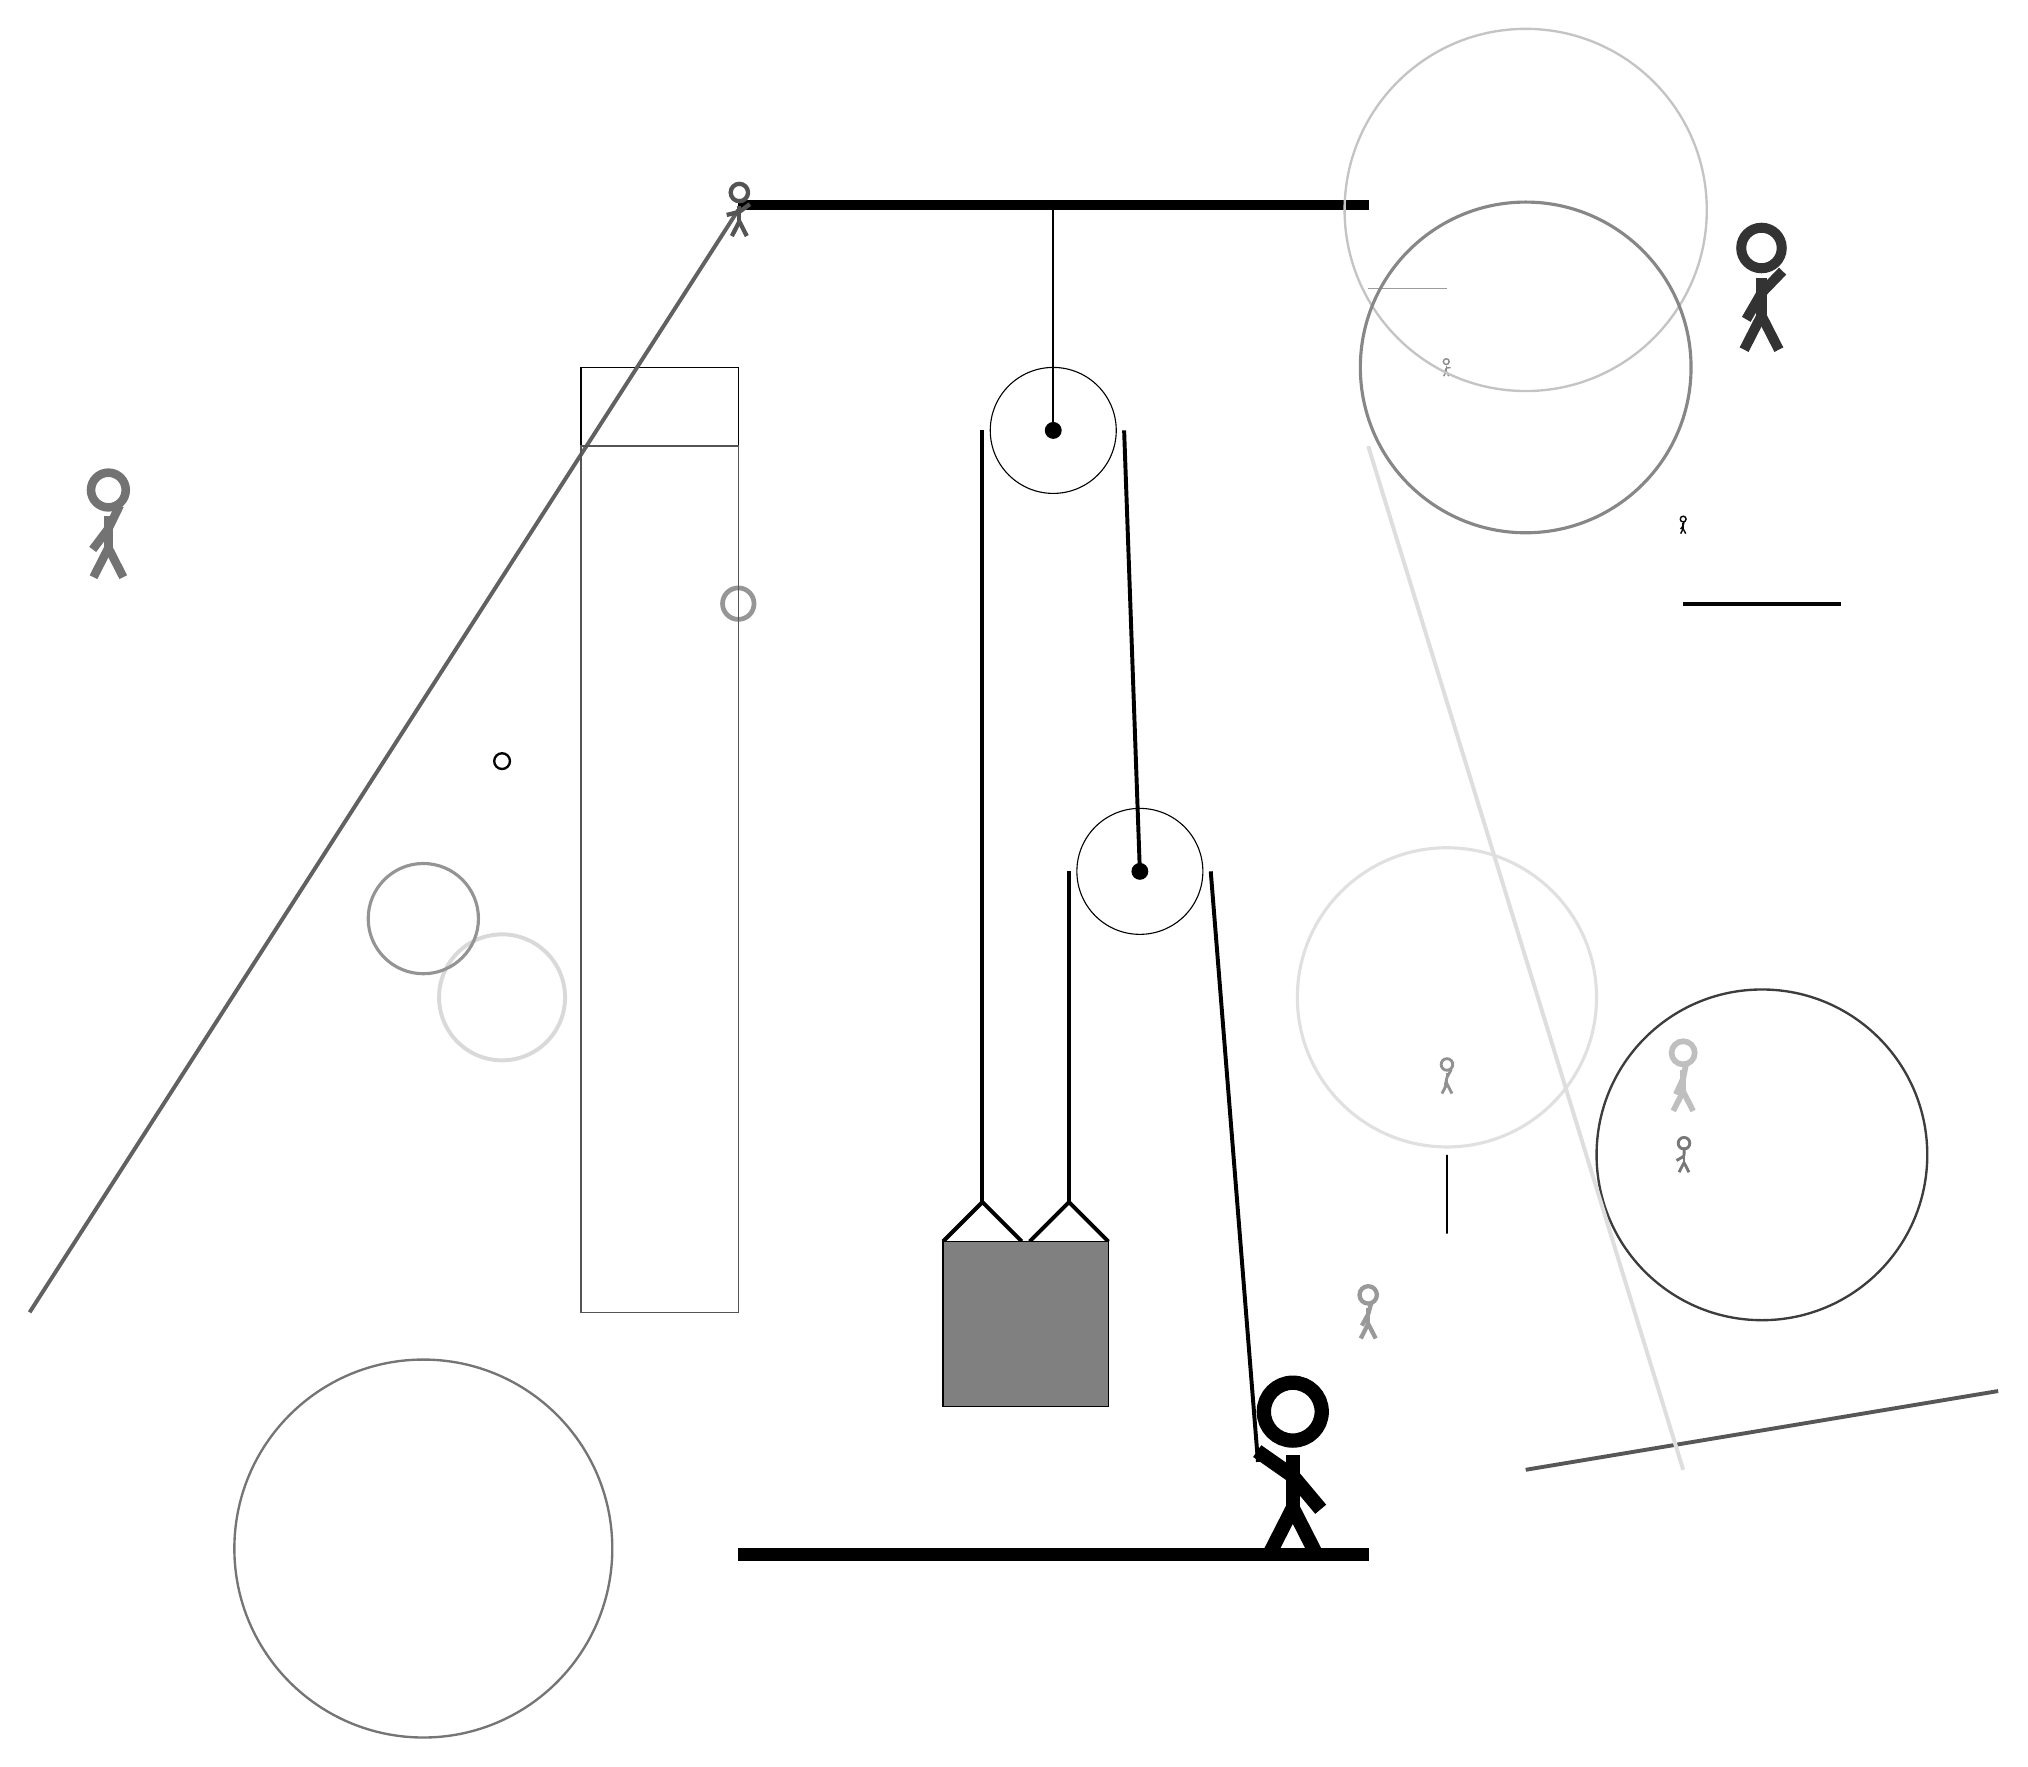
\begin{tikzpicture}
			%%%%% START %%%%%
			
			\draw[fill=black] (-2, 14) rectangle (6, 14.125);
			
			\draw (2, 11.2) circle (0.8);
			\draw[fill=black] (2, 11.2) circle (0.1);
			\draw[thick] (2, 11.2) -- (2, 14);
			
			\draw (3.1, 5.6) circle (0.8);
			\draw[fill=black] (3.1, 5.6) circle (0.1);
			
			\draw[line width = 0.5mm]  (0.6, 0.9) -- (1.1, 1.4) -- (1.6, 0.9);
			\draw[line width = 0.5mm]  (1.7, 0.9) -- (2.2, 1.4) -- (2.7, 0.9);
			\draw[fill=black!50] (0.6, 0.9) rectangle (2.7, -1.2);
			
			\draw[line width = 0.5mm] (1.1, 11.2) -- (1.1, 1.4);
			\centerarc[line width = 0.5mm](2, 11.2)(0:180:0.9);
			\draw[line width = 0.5mm] (2.9, 11.2) -- (3.1, 5.6);
			\draw[line width = 0.5mm] (2.2, 5.6) -- (2.2, 1.4);
			\centerarc[line width = 0.5mm](3.1, 5.6)(0:180:0.9);
			\draw[line width = 0.5mm] (4.0, 5.6) -- (4.6, -1.9);
			
			\draw[line width=0.2mm, color=black!100] (7, 2) rectangle (7, 1);
			
			\node[line width=0.6mm, color=black!53] at (10, 2) {\Strichmaxerl[2][31][88]};
			\draw [line width=0.3mm, color=black!76](11, 2) circle (2.1);
			\node[line width=0.5mm, color=black!43] at (7, 3) {\Strichmaxerl[2][78][61]};
			\node[line width=0.3mm, color=black!46] at (7, 12) {\Strichmaxerl[1][71][7]};
			\draw [line width=0.6mm, color=black!41](-2, 9) circle (0.2);
			
			\draw [line width=0.5mm, color=black!15](-5, 4) circle (0.8);
			
			\draw [line width=0.3mm, color=black!23](8, 14) circle (2.3);
			\node[line width=0.5mm, color=black!80] at (11, 13) {\Strichmaxerl[7][60][46]};
			\draw [line width=0.3mm, color=black!54](-6, -3) circle (2.4);
			
			\node[line width=0.7mm, color=black!25] at (10, 3) {\Strichmaxerl[4][65][79]};
			
			\draw [line width=0.3mm, color=black!99](-5, 7) circle (0.1);
			\draw[line width=0.2mm, color=black!99] (-2, 0) rectangle (-4, 12);
			
			\node[line width=0.2mm, color=black!96] at (10, 10) {\Strichmaxerl[1][56][77]};
			\draw[line width=0.2mm, color=black!39] (7, 13) rectangle (6, 13);
			\draw[line width=0.5mm, color=black!66](8, -2) -- (14, -1);
			
			\node[line width=0.3mm, color=black!40] at (6, 0) {\Strichmaxerl[3][61][75]};
			\draw [line width=0.4mm, color=black!42](-6, 5) circle (0.7);
			\draw [line width=0.4mm, color=black!12](7, 4) circle (1.9);
			
			\draw[line width=0.5mm, color=black!62](-2, 14) -- (-11, 0);
			\draw[line width=0.2mm, color=black!67] (-4, 0) rectangle (-2, 11);
			
			\node[line width=0.3mm, color=black!55] at (-10, 10) {\Strichmaxerl[6][53][64]};
			\draw[line width=0.5mm, color=black!98](10, 9) -- (12, 9);
			\draw[line width=0.5mm, color=black!13](6, 11) -- (10, -2);
			\node[line width=0.5mm, color=black!67] at (-2, 14) {\Strichmaxerl[3][14][36]};
			
			\draw [line width=0.4mm, color=black!47](8, 12) circle (2.1);
			
			\node at (5, -2) {\Strichmaxerl[10][-35][-50]};
			
			\draw[fill=black] (-2, -3) rectangle (6, -3.15);
			
			%%%%% END %%%%%
		\end{tikzpicture}
	\end{figure}	
\end{document}